\documentclass[chapterprefix=false]{report}
\setlength{\oddsidemargin}{0 in}
\setlength{\evensidemargin}{0 in}
\setlength{\topmargin}{0 in}
\setlength{\textwidth}{5.7 in}
\setlength{\textheight}{8.0 in}
\setlength{\headsep}{0.75 in}
\setlength{\parindent}{0.3 in}
\setlength{\parskip}{0.1 in}

\usepackage{titlesec}

\titleformat{\chapter}{\huge}{\thechapter.}{20pt}{\huge}

\usepackage{epsf}
\usepackage{pseudocode}
\usepackage{amssymb}
\usepackage{mathtools}
\usepackage{amsmath}
\usepackage{algorithm}
\usepackage[noend]{algpseudocode}
\usepackage{textcomp}
\usepackage{tikz}
\usepackage{csquotes}
\usepackage{graphicx}
\usepackage{enumitem}
\usepackage{seqsplit}
\graphicspath{{photos/}}

\usepackage{url}
\usepackage{cite}
\usepackage[parfill]{parskip}
%\usepackage{natbib}
%\bibliographystyle{unsrtnat}

\usetikzlibrary{arrows}
\tikzset{
    vertex/.style={circle,draw,minimum size=1.5em},
    edge/.style={->,> = latex'}
}

\makeatletter
\def\BState{\State\hskip-\ALG@thistlm}
\makeatother

\DeclarePairedDelimiter\ceil{\lceil}{\rceil}
\DeclarePairedDelimiter\floor{\lfloor}{\rfloor}

% \usepackage{times}
% \usepackage{mathptm}

\def\O{\mathop{\smash{O}}\nolimits}
\def\o{\mathop{\smash{o}}\nolimits}
\newcommand{\e}{{\rm e}}
\newcommand{\R}{{\bf R}}
\newcommand{\Z}{{\bf Z}}
\newcommand{\h}{1.2}

\DeclareMathOperator*{\argmin}{arg\,min}
\DeclareMathOperator*{\argmax}{arg\,max}
 
\begin{document}
 
\tableofcontents{}
 
\chapter{Introduction}
 
\section{In-game Sports Analytics}

$\newline$
``The win probability graphic/discussion on ESPN is literally taking a sword and sticking it through the chest of any fun left in baseball''
\\[5pt]
\centerline{{ --- Kenny Ducey (@KennyDucey) April 2, 2017}}

$\newline$
``ESPN showing win probability is extremely good. Next up, run expectancy!''
\\[5pt]
\centerline{{\rm --- Neil Weinberg (@NeilWeinberg44) April 4, 2017}}

``Thank the Lord we have the ESPN Win Probability stat to tell us the team that's ahead has a good chance to win.''
\\[5pt]
\centerline{{\rm --- Christian Schneider (@Schneider\_CM) April 17, 2017}}

In recent years, win probability has become increasingly prevalent in sports broadcasting. Brian Burke, an NFL commentator, has posted live win-probability graphs of NFL playoff games on his website for the past few years. Earlier this year, ESPN began to post win probabilities atop the score box in televised Major League Baseball games. Despite mixed reactions from fans, as shown above, these developments represent a transition in sports broadcasting's modern narrative. 

%..Make an argument for the value of in-match forecasting, despite angry reactions..

A win probability from any score line communicates how much one team or player is favored to win. While one can produce this from any model of choice, the field strives to produce the most well-informed estimate of how likely a player is to win the match. With the recent proliferation of online betting, in-match win probability dictates an entire market of its own. Betfair's platform  matched over 40 million Euros during the 2011 French Open Final \cite{Huang2011}; other high-profile matches often draw comparable volume over betting exchanges. While the majority of tennis prediction papers concern pre-match prediction, around 80$\%$ of online betting occurs while matches are in progress \cite{Sipko2015}. Clearly, in-match win probability is of great concern to all participants in this betting market. 


%While tennis has yet to broadcast win probabilities, 

%demonstrates an individual model’s most informed guess at how likely a player is to win the match

%Drawing upon past research and exploring new methods, this paper searches for the most effective approach to in-match forecasting.

\section{History of Tennis Forecasting}
Plenty of research on tennis match prediction exists over the past twenty years. Klaassen and Magnus tested the assumption that points in a tennis match are independent and identically distributed \cite{KlaassenandMagnus2001}. Under this assumption, they construct a hierarchical Markov model in conjunction with tennis’ scoring system. From this model, they offer an analytical equation for match-win probability from any score, given each individual player's probability of winning a point on serve \cite{Klaassen2003}.  Barnett and Clarke then offer a method of estimating each player's serve probability from historical data \cite{BarnettandClarke2005}. Years later, Bevc proposed updating each these serve probabilities with a beta distribution between each point and computing the corresponding win probability with the above model \cite{Bevc2015}. Recently, Kovalchik assessed performance of 11 different pre-match prediction models on all tour-level ATP matches in 2014 \cite{Kovalchik2016}.

Over the past several years, Jeff Sackmann (offer footnote to website) has released the largest publicly available library of tennis datasets via github. This collection contains match summaries of every ATP and WTA match in the Open Era, point-by-point summaries of nearly 100,000 tour-level and satellite matches, and a crowd-sourced match-charting project spanning over 3000 matches, where volunteers record each shot’s type and direction over an entire match. While 538 and Kovalchik use Jeff Sackmann’s match data to generate elo ratings, none of the aforementioned papers have tested models with his point-by-point dataset.

As past papers have spanned several decades, datasets and model evaluation are not consistent. Klaassen and Magnus' original point-based model and Bevc's beta experiments both apply methods to around 500 Wimbledon matches from 1991-94. Barnett explores point-based models in great depth, yet primarily applies them to a single marathon match between Andy Roddick and Younes El Aynaoui from the 2002 Australian Open \cite{Barnett2006}. Except for Bevc, none of these papers attempt to obtain an overall assessment of in-game match prediction with metrics such as accuracy or cross-entropy. While Bevc does record accuracy of results over 500 Wimbledon matches, he only reports accuracy of predictions in the third set and onwards, a subset of the entire dataset. In other words, no one has taken all in-game prediction models and tested them at a large scale. For this reason, I will test all relevant in-match prediction methods on thousands of matches within the past seven years.

%However, Jeff Sackmann has recently released the largest publicly available tennis dataset via github. This collection contains match summaries of every ATP and WTA match in the Open Era, point-by-point summaries of nearly 100,000 matches—both tour-level and satellite--and a crowd-sourced match-charting project spanning 2800 matches, where volunteers record each shot’s type and direction in every point. While 538 and Kovalchik use Jeff Sackmann’s match data to refine their own elo system for pre-match prediction, no papers on in-match prediction have used his point-by-point dataset. With over 10,000 ATP and WTA tour-level matches from 2010-2017, I compare existing approaches side-by-side and explore new methods to in-match prediction.  Just as Kovalchik does with pre-match prediction models, I attempt to find the GOAT (greatest of all-time) of in-match prediction models.

This paper combines elo ratings, a wealth of data, and current technology to provide a similar survey of which in-match prediction methods perform the best. I build upon past research by testing variations of previous state-of-the-art methods, and applying several new concepts to these datasets, from successful probability models in football and baseball, to state exploration via hidden Markov Models.

 (Can reference older sports forecasting mentioned in Nettleton and Lock...)

 
\section{Match/Point-by-Point Datasets}
 
 This project uses two different types of datasets: one with match summary statistics and one with point-by-point information. Both are publicly available on github, courtesy of Jeff Sackmann (\url{https://github.com/JeffSackmann}). We primarily use the matches dataset under ``\texttt{tennis\_atp}'' to test pre-match prediction methods. This dataset covers over 150,000 tour-level matches, dating back to 1968. Features include player qualities, such as nationality or dominant hand, as well as match statistics, like serve/return points won.
 
 
 The data in ``\texttt{tennis\_pointbypoint}'' offers more granular detail about a single match's point progression. Each match contains a string listing the order in which players won points and switched serve. As the ATP does not publicly list point-by-point summaries, this information was presumably extracted from a betting website.

\section{Implementation}

With the above datasets serving as a basis for this project, thorough re-formatting of the data was required in order to connect point-by-point strings to their corresponding rows in the match dataset.

As both datasets included player names, year, and score, we connected matches across datasets with a hashing scheme \footnote{eg. hash(matchX) = ``Roger Federer Tomas Berdych 2012 3-6 7-5 7-5''}. Due to observed inconsistencies, we canonicalized player names between match and point-by-point datasets $\footnote{eg. ``Stan Wawrinka'' $\rightarrow$ ``Stanislas Wawrinka'', ``Federico Del Bonis'' $\rightarrow$ ``Federico Delbonis''}$ in order to maximize the number of available matches with point-by-point summaries. As a portion of the point-by-point summaries are from satellite events, we were able to match around 10,600/12,000 point-by-point strings to their respective tour-level matches. Then, we could then associate information generated from the match dataset's entirety (elo ratings, year-long adjusted serve stats, etc) with these point-by-point strings.

To view this process in more depth, or access any of the resulting datasets, visit \url{https://github.com/jgollub1/tennis_match_prediction}. Implementations of each method in this project, and instructions on how to generate all relevant statistics, are also provided.


\chapter{Scoring}
Tennis' scoring system consists of three levels: sets, games, and points. Consider a tennis match between two entities, $p_i$ and $p_j$. We can represent any score as $(s_i,s_j),(g_i,g_j),({x}_i,{x}_j)$ where $i$ is serving and $s_k,g_k,x_k$ represent player $k$'s score in sets, games, and points, respectively. The players alternate serve each game and continue until someone clinches the match by winning two sets (best-of-three) or three sets (best-of-five) $\footnote{The best-of-five format is typically reserved for men's grand slam and Davis Cup events}$.

The majority of in-play tennis models utilize a hierarchical Markov Model, which embodies the levels in tennis' scoring system. Barnett formally defines a representation for scores in tennis \cite{BarnettandClarke2002}. With $p_i$ and $p_j$ winning points on serve with probabilities $f_{ij},f_{ji}$, each in-match scoreline $(s_i,s_j),(g_i,g_j),({x}_i,{x}_j)$ progresses to one of its two neighbors $(s_i,s_j),(g_i,g_j),({x}_i+1,{x}_j)$ and $(s_i,s_j),(g_i,g_j),({x}_i,{x}_j+1)$ with transition probabilities dependent on the current server. Assuming all points in a match are $iid$, we can then use the below model to recursively determine win probability:

\begin{center}
$P_m(s_i,s_j,g_i,g_j,{x}_i,{x}_j)$ = probability that $p_i$ wins the match when serving from this scoreline

$P_m(s_i,s_j,g_i,g_j,{x}_i,{x}_j) = f_{ij}*P_m(s_i,s_j,g_i,g_j,{x}_i+1,{x}_j) + (1-f_{ij}) P_m(s_i,s_j,g_i,g_j,{x}_i,{x}_j+1)$
\end{center}
In the following sections, we specify boundary values to each level of our hierarchical model. 

%With these specifications, we can analytically compute win probability at any point in the match.


\section{Modeling games}

Within a game, either $p_i$ or $p_j$ serves every point. Every game starts at (0,0) and to win a game, a player must win four or more points by a margin of at least two $\footnote{While tennis officially  refers to a game's first three points as 15,30,40 we will call them 1,2,3 for simplicity's sake}$. Consequently, all games with valid scores $(x_i,x_j)$ where $x_i+x_j$ \textgreater $6; |x_i-x_j| \leq 1$ are reduced to (3,3), (3,2), or (2,3). Furthermore, the win probability at (3,3) can be calculated directly. From (3,3), the server wins the next two points with probability $f_{ij}^2$, the returner wins the next two points with probability $(1-f_{ij})^2$, or both players split the two points and return to (3,3) with probability $2f_{ij}(1-f_{ij})$. Relating the game's remainder to a geometric sequence, we find $P_g(3,3) = \frac{f_{ij}^2}{f_{ij}^2+(1-f_{ij})^2}$.

Possible sequences of point scores in a game:

a - player $i$ wins the following point

b - player $j$ wins the following point

\begin{tikzpicture} [scale=1]
\tikzset{VertexStyle/.style = {shape = circle,inner sep=0x}}
\node[vertex] (1) at (0,0) {$0,0$};
\node[vertex] (2) at (2,.8) {$1,0$};
\node[vertex] (3) at (2,-.8) {$0,1$};
\node[vertex] (4) at (4,0) {$1,1$};
\node[vertex] (7) at (4,1.6) {$2,0$};
\node[vertex] (8) at (4,-1.6) {$0,2$};
\node[vertex] (5) at (6,.8) {$2,1$};
\node[vertex] (6) at (6,-.8) {$1,2$};
\node[vertex] (9) at (6,2.4) {$3,0$};
\node[vertex] (10) at (6,-2.4) {$0,3$};
\node[vertex] (11) at (8,1.6) {$3,1$};
\node[vertex] (12) at (8,-1.6) {$1,3$};
\node[vertex] (13) at (8,0) {$2,2$};

\node[vertex] (14) at (12,3.2) {$G_1$};
\node[vertex] (15) at (12,-3.2) {$G_1^{c}$};
\node[vertex] (16) at (10,.8) {$3,2$};
\node[vertex] (17) at (10,-.8) {$2,3$};
\node[vertex] (18) at (12,0) {$3,3$};

\draw[edge] (1) -- (2) node[midway, above] {$a$};
\draw[edge] (1) -- (3) node[midway, above] {$b$};
\draw[edge] (2) -- (4) node[midway, above] {$b$};
\draw[edge] (3) -- (4) node[midway, above] {$a$};
\draw[edge] (2) -- (7) node[midway, above] {$a$};
\draw[edge] (3) -- (8) node[midway, above] {$b$};
\draw[edge] (4) -- (5) node[midway, above] {$a$};
\draw[edge] (4) -- (6) node[midway, above] {$b$};
\draw[edge] (7) -- (9) node[midway, above] {$a$};
\draw[edge] (7) -- (5) node[midway, above] {$b$};
\draw[edge] (8) -- (6) node[midway, above] {$a$};
\draw[edge] (8) -- (10) node[midway, above] {$b$};
\draw[edge] (9) -- (11) node[midway, above] {$b$};
\draw[edge] (10) -- (12) node[midway, above] {$a$};
\draw[edge] (5) -- (11) node[midway, above] {$a$};
\draw[edge] (6) -- (12) node[midway, above] {$b$};
\draw[edge] (5) -- (13) node[midway, above] {$b$};
\draw[edge] (6) -- (13) node[midway, above] {$a$};
\draw[edge] (13) -- (16) node[midway, above] {$a$};
\draw[edge] (13) -- (17) node[midway, above] {$b$};
\draw[edge] (11) -- (16) node[midway, above] {$b$};
\draw[edge] (12) -- (17) node[midway, above] {$a$};
\draw[edge] (16) -- (18) node[midway, above] {$b$};
\draw[edge] (17) -- (18) node[midway, above] {$a$};
\draw[edge] (9) -- (14) node[midway, above] {$a$};
\draw[edge] (11) -- (14) node[midway, above] {$a$};
\draw[edge] (16) -- (14) node[midway, above] {$a$};
\draw[edge] (10) -- (15) node[midway, above] {$b$};
\draw[edge] (12) -- (15) node[midway, above] {$b$};
\draw[edge] (17) -- (15) node[midway, above] {$b$};
\draw[->, xshift=11.3cm, yshift=1cm] (18) to [bend right=50] (16) node[ sloped,midway,above] {$a$};
\draw[->, xshift=11.3cm, yshift=-1cm] (18) to [bend left=50] (17) node[ sloped,midway,above] {$b$};

\end{tikzpicture}

Boundary values:

\begin{equation}
    P_g(x_i,x_j) 
    \begin{cases}
      1, & \text{if}\ x_1=4,x_2 \leq 2 \\
      0, & \text{if}\ x_2=4,x_1 \leq 2 \\
      \cfrac{f_{ij}^2}{f_{ij}^2+(1-f_{ij})^2}, & \text{if}\ x_1=x_2=3 \\
      f_{ij}*P_g(s_i,s_j,g_i,g_j,{x}_i+1,{x}_j) + (1-f_{ij}) P_g(s_i,s_j,g_i,g_j,{x}_i,{x}_j+1), & \text{otherwise}\ \\
      
    \end{cases}
  \end{equation}

With the above specifications, we can efficiently compute player $i$'s win probability from any score $P_g(x_i,x_j)$.

\section{Modeling sets}

Within a set, $p_i$ or $p_j$ alternate serve every game. Every set starts at (0,0). To win a set, a player must win six or more games by a margin of at least two. If the set score $(6,6)$ is reached, a special tiebreaker game is played to determine the outcome of the match.

Possible sequences of point scores in a game:

$a$ - player 1 wins the following game

$b$ - player 2 wins the following game

$a'$ - player 1 wins the tiebreaker game

$b'$ - player 2 wins the tiebreaker game

\begin{tikzpicture} [scale=.7]
\tikzset{VertexStyle/.style = {shape = circle,inner sep=0x}}
\node[vertex] (1) at (0,0) {$0,0$};
\node[vertex] (2) at (2,\h) {$1,0$};
\node[vertex] (3) at (2,-\h) {$0,1$};
\node[vertex] (4) at (4,2*\h) {$2,0$};
\node[vertex] (5) at (4,0) {$1,1$};
\node[vertex] (6) at (4,-2*\h) {$0,2$};
\node[vertex] (7) at (6,3*\h) {$3,0$};
\node[vertex] (8) at (6,\h) {$2,1$};
\node[vertex] (9) at (6,-\h) {$1,2$};
\node[vertex] (10) at (6,-3*\h) {$0,3$};
\node[vertex] (11) at (8,4*\h) {$4,0$};
\node[vertex] (12) at (8,2*\h) {$3,1$};
\node[vertex] (13) at (8,0) {$2,2$};
\node[vertex] (14) at (8,-2*\h) {$1,3$};
\node[vertex] (15) at (8,-4*\h) {$0,4$};
\node[vertex] (16) at (10,5*\h) {$5,0$};
\node[vertex] (17) at (10,3*\h) {$4,1$};
\node[vertex] (18) at (10,\h) {$3,2$};
\node[vertex] (19) at (10,-\h) {$2,3$};
\node[vertex] (20) at (10,-3*\h) {$1,4$};
\node[vertex] (21) at (10,-5*\h) {$0,5$};
\node[vertex] (22) at (18,6*\h) {$S_1$};
\node[vertex] (23) at (12,4*\h) {$5,1$};
\node[vertex] (24) at (12,2*\h) {$4,2$};
\node[vertex] (25) at (12,0) {$3,3$};
\node[vertex] (26) at (12,-2*\h) {$2,4$};
\node[vertex] (27) at (12,-4*\h) {$1,5$};
\node[vertex] (28) at (18,-6*\h) {$S_1^c$};
\node[vertex] (29) at (14,3*\h) {$5,2$};
\node[vertex] (30) at (14,\h) {$4,3$};
\node[vertex] (31) at (14,-\h) {$3,4$};
\node[vertex] (32) at (14,-3*\h) {$2,5$};
\node[vertex] (33) at (16,2*\h) {$5,3$};
\node[vertex] (34) at (16,0) {$4,4$};
\node[vertex] (35) at (16,-2*\h) {$3,5$};
\node[vertex] (36) at (18,\h) {$5,4$};
\node[vertex] (37) at (18,-\h) {$4,5$};
\node[vertex] (38) at (20,0) {$5,5$};
\node[vertex] (39) at (22,\h) {$6,5$};
\node[vertex] (40) at (22,-\h) {$5,6$};
\node[vertex] (41) at (24,0) {$6,6$};



\draw[edge] (1) -- (2) node[midway, above] {$a$};
\draw[edge] (1) -- (3) node[midway, above] {$b$};
\draw[edge] (2) -- (4) node[midway, above] {$b$};
\draw[edge] (2) -- (5) node[midway, above] {$a$};
\draw[edge] (3) -- (5) node[midway, above] {$a$};
\draw[edge] (3) -- (6) node[midway, above] {$b$};
\draw[edge] (4) -- (7) node[midway, above] {$a$};
\draw[edge] (4) -- (8) node[midway, above] {$b$};
\draw[edge] (5) -- (8) node[midway, above] {$a$};
\draw[edge] (5) -- (9) node[midway, above] {$b$};
\draw[edge] (6) -- (9) node[midway, above] {$a$};
\draw[edge] (6) -- (10) node[midway, above] {$b$};
\draw[edge] (7) -- (11) node[midway, above] {$a$};
\draw[edge] (7) -- (12) node[midway, above] {$b$};
\draw[edge] (8) -- (12) node[midway, above] {$a$};
\draw[edge] (8) -- (13) node[midway, above] {$b$};
\draw[edge] (9) -- (13) node[midway, above] {$a$};
\draw[edge] (9) -- (14) node[midway, above] {$b$};
\draw[edge] (10) -- (14) node[midway, above] {$a$};
\draw[edge] (10) -- (15) node[midway, above] {$b$};
\draw[edge] (11) -- (16) node[midway, above] {$a$};
\draw[edge] (11) -- (17) node[midway, above] {$b$};
\draw[edge] (12) -- (17) node[midway, above] {$a$};
\draw[edge] (12) -- (18) node[midway, above] {$b$};
\draw[edge] (13) -- (18) node[midway, above] {$a$};
\draw[edge] (13) -- (19) node[midway, above] {$b$};
\draw[edge] (14) -- (19) node[midway, above] {$a$};
\draw[edge] (14) -- (20) node[midway, above] {$b$};
\draw[edge] (15) -- (20) node[midway, above] {$a$};
\draw[edge] (15) -- (21) node[midway, above] {$b$};
\draw[edge] (16) -- (22) node[midway, above] {$a$};
\draw[edge] (16) -- (23) node[midway, above] {$b$};
\draw[edge] (17) -- (23) node[midway, above] {$a$};
\draw[edge] (17) -- (24) node[midway, above] {$b$};
\draw[edge] (18) -- (24) node[midway, above] {$a$};
\draw[edge] (18) -- (25) node[midway, above] {$b$};
\draw[edge] (19) -- (25) node[midway, above] {$a$};
\draw[edge] (19) -- (26) node[midway, above] {$b$};
\draw[edge] (20) -- (26) node[midway, above] {$a$};
\draw[edge] (20) -- (27) node[midway, above] {$b$};
\draw[edge] (21) -- (27) node[midway, above] {$a$};
\draw[edge] (21) -- (28) node[midway, above] {$b$};
\draw[edge] (23) -- (22) node[midway, above] {$a$};
\draw[edge] (23) -- (29) node[midway, above] {$b$};
\draw[edge] (24) -- (29) node[midway, above] {$a$};
\draw[edge] (24) -- (30) node[midway, above] {$b$};
\draw[edge] (25) -- (30) node[midway, above] {$a$};
\draw[edge] (25) -- (31) node[midway, above] {$b$};
\draw[edge] (26) -- (31) node[midway, above] {$a$};
\draw[edge] (26) -- (32) node[midway, above] {$b$};
\draw[edge] (27) -- (32) node[midway, above] {$a$};
\draw[edge] (27) -- (28) node[midway, above] {$b$};
\draw[edge] (29) -- (22) node[midway, above] {$a$};
\draw[edge] (29) -- (33) node[midway, above] {$b$};
\draw[edge] (30) -- (33) node[midway, above] {$a$};
\draw[edge] (30) -- (34) node[midway, above] {$b$};
\draw[edge] (31) -- (34) node[midway, above] {$a$};
\draw[edge] (31) -- (35) node[midway, above] {$b$};
\draw[edge] (32) -- (35) node[midway, above] {$a$};
\draw[edge] (32) -- (28) node[midway, above] {$b$};
\draw[edge] (33) -- (22) node[midway, above] {$a$};
\draw[edge] (33) -- (36) node[midway, above] {$b$};
\draw[edge] (34) -- (36) node[midway, above] {$a$};
\draw[edge] (34) -- (37) node[midway, above] {$b$};
\draw[edge] (35) -- (37) node[midway, above] {$a$};
\draw[edge] (35) -- (28) node[midway, above] {$b$};
\draw[edge] (36) -- (22) node[midway, left] {$a$};
\draw[edge] (36) -- (38) node[midway, above] {$b$};
\draw[edge] (37) -- (38) node[midway, above] {$a$};
\draw[edge] (37) -- (28) node[midway, right] {$b$};
\draw[edge] (38) -- (39) node[midway, above] {$a$};
\draw[edge] (38) -- (40) node[midway, above] {$b$};
\draw[edge] (39) -- (22) node[midway, above] {$a$};
\draw[edge] (39) -- (41) node[midway, above] {$b$};
\draw[edge] (40) -- (41) node[midway, above] {$a$};
\draw[edge] (40) -- (28) node[midway, above] {$b$};

\draw[->, xshift=20cm,yshift=6.35cm] (41) to [bend right=30] (22) node[sloped,midway,above,scale=1.4] {$a'$};
\draw[->, xshift=20cm,yshift=-6.35cm] (41) to [bend left=30] (28) node[sloped,midway,above,scale=1.4] {$b'$};


\end{tikzpicture}

Boundary values:
\begin{equation}
    P_s(g_1,g_2) 
    \begin{cases}
      1, & \text{if}\ g_1 \geq 6,g_1-g_2 \geq 2 \\
      0, & \text{if}\ g_2 \geq 6,g_2-g_1 \geq 2 \\
      P_{tb}(s_1,s_2), & \text{if}\ g_1=g_2=6 \\
      P_g(0,0)(1-P_s(g_2,g_1+1))+(1-P_g(0,0))(1-P_s(g_2+1,g_1)), & \text{otherwise}\ \\
    \end{cases}
  \end{equation}

See appendix for the tiebreak game's corresponding diagram**

\section{Modeling a tie-break game}


\section{Modeling a best-of-three match}


a - player 1 wins the following set

b - player 2 wins the following set

\begin{tikzpicture} [scale=1]
\node[vertex] (1) at (0,0) {$0,0$};
\node[vertex] (2) at (2,1) {$1,0$};
\node[vertex] (3) at (2,-1) {$0,1$};
\node[vertex] (4) at (4,0) {$1,1$};
\node[vertex] (5) at (6,1) {$W_1$};
\node[vertex] (6) at (6,-1) {$W_1^{c}$};

\draw[edge] (1) -- (2) node[midway, above] {$a$};
\draw[edge] (1) -- (3) node[midway, above] {$b$};
\draw[edge] (2) -- (4) node[midway, above] {$b$};
\draw[edge] (3) -- (4) node[midway, above] {$a$};
\draw[edge] (2) -- (5) node[midway, above] {$a$};
\draw[edge] (3) -- (6) node[midway, above] {$b$};
\draw[edge] (4) -- (5) node[midway, above] {$a$};
\draw[edge] (4) -- (6) node[midway, above] {$b$};

\end{tikzpicture}

Boundary values:
\begin{equation}
    P_m(s_1,s_2) 
    \begin{cases}
      1, & \text{if}\ g_1 \geq 2 \\
      0, & \text{if}\ g_2 \geq 2 \\
      P_s(0,0)(P_m(s_1+1,s_2))+(1-P_s(0,0))(P_m(s_1,s_2+1)), & \text{otherwise}\ \\
    \end{cases}
  \end{equation}


\section{Win Probability Equation}
Combining the above equations, we can recursively calculate win probability with player $i$ serving from $(s_i,s_j,g_i,g_j,{x}_i,{x}_j)$ as:

$P_m(s_i,s_j,g_i,g_j,{x}_i,{x}_j) = f_{ij}*P_m(s_i,s_j,g_i,g_j,{x}_i+1,{x}_j) + (1-f_{ij}) P_m(s_i,s_j,g_i,g_j,{x}_i,{x}_j+1) \newline 
= P_g(x_i,x_j)*(1-P_m(s_j,s_i,g_j,g_i+1,0,0)) + (1-P_g(x_i,x_j))*(1-P_m(s_j,s_i,g_j+1,g_i,0,0)) \newline
= 
P_g(x_i,x_j)*(1-(P_s(g_j,g_i+1)*P_m(s_j+1,s_i)+(1-P_s(g_j,g_i+1))*P_m(s_j,s_i+1)) + (1-P_g(x_i,x_j))*(1-(P_s(g_j+1,g_i)*P_m(s_j+1,s_i)+(1-P_s(g_j+1,g_i))*P_m(s_j,s_i+1)) = ...$

Thanks to the boundary values at each level, we can programmatically compute this equation.

\chapter{Pre-game Match Prediction}

\section{Overview}
Before play has started, an in-match prediction model cannot draw on information from the match itself. Then, before a match between $p_i$ and $p_j$ commences, the most well-informed pre-match forecast $\hat{\pi}_{ij}(t)$ should serve as a basis for prediction. Therefore, we first explore pre-match models as a starting point for in-match prediction.

Earlier this year, Kovalchik released a survey of eleven different pre-match prediction models, assessing them side-by-side in accuracy, log-loss, calibration, and discrimination. 538's elo-based model and the Bookmaker Consensus Model performed the best. Elo-based prediction incorporates player $i$ and $j$'s entire match histories, while the BCM model incorporates all information encoded in the betting market. As we will later back-test effective in-match models against market data, we first explore all pre-match prediction methods that do not employ market data.

%However, the paper leaves out a point-based method  devised by Klaassen and Magnus that derives serving probabilities from historical player data (combining player outcomes).

\section{Elo Ratings}
Elo was originally developed as a head-to-head rating system for chess players (1978). Recently, 538's elo variant has gained prominence in the media. For a match at time $t$ between $p_i$ and $p_j$ with elo ratings $E_i(t)$ and $E_j(t)$, $p_i$ is forecasted to win with probability:

\begin{center}
$\hat{\pi}_{ij}(t) = (1 + 10^\frac{E_j(t)-E_i(t)}{400})^{-1}$
\end{center}

$p_i$'s rating for the following match $t+1$ is then updated accordingly:

\begin{center}
$E_i(t+1) = E_i(t) + K_{it}*(W_i(t)-\hat{\pi}_{ij}(t))$
\end{center}

$W_i(t)$ is an indicator for whether $p_i$ won the given match, while $K_{it}$ is the learning rate for $p_i$ at time $t$. According to 538's analysts, elo ratings perform optimally when allowing $K_{it}$ to  decay slowly over time (How We're Predicting). With $m_i(t)$ representing the $p_i$'s career matches played at time $t$ we update our learning rate:

\begin{center}
$K_{it} = \frac{250}{(5+m(t))^{.4}} $
\end{center}

This variant updates a player's elo most quickly when we have no information about a player and makes smaller changes as $m_i(t)$ accumulates. To apply this elo rating method to our dataset, we initalize each player's elo rating at $E_i(0)=1500$ and match history $m_i(0)=0$. Then, we iterate through all tour-level matches from 1968-2017 $\footnote{tennis' Open Era began in 1968, when professionals were allowed to enter grand slam tournaments. Before then, only amateurs played these events}$ in chronological order, storing $E_i(t),E_j(t)$ for each match and updating each player's elo accordingly.

\section{ATP Rank}
While Klaassen incorporated ATP rank into his prediction model \cite{Klaassen2003}, Kovalchik and 538 concur that elo outperforms ranking-based methods. On ATP match data from 2010-present, we found:

\begin{center}
\begin{tabular}{ |c|c| } 
 \hline
 method & accuracy
   \\ 
 \hline
  ATP Rank & 66.5 \%
  \\ 
 \hline
  Standard elo & 69.0 \%
  \\ 
 \hline
\end{tabular}
\end{center}

Considering its superiority to ATP rank in recent years, models in this paper use elo ratings to represent a player's ability in place of official tour rank.

\section{Point-based Model}
The hierarchical Markov Model offers an analytical solution to win probability $\hat{\pi}_{ij}(t)$ between players $p_i$ and $p_j$, given serving probabilities $f_{ij}$,$f_{ji}$. This hinges on the Markov assumption that transition probabilities from any state only depend on the current state. In other words, all points are independent and the probability of winning a given point only depends on the current server. While this is counter-intuitive, Klaassen and Magnus demonstrated that deviations from the iid assumption within matches are small enough to reasonably justify point-based models \cite{KlaassenandMagnus2001}. Later on, Barnett and Clarke demonstrated a method to estimate $f_{ij},f_{ji}$, given players' historical serve/return averages \cite{BarnettandClarke2005}.

%This model assumes that all points in a tennis match are independent and identically distributed with respect to each server's ability

%outline a way to estimate each player's serving probability from historical serve and return data. 

\begin{center}
$f_{ij} = f_t + (f_i-f_{av})-(g_j-g_{av})$
%\newline

$f_{ji} = f_t + (f_j-f_{av})-(g_i-g_{av})$
\end{center}

Each player's serve percentage is a function of their own serving ability and their opponent's returning ability. $f_t$ denotes the average serve percentage for the match's given tournament, while $f_i,f_j$ and $g_i,g_j$ represent player $i$ and $j$'s percentage of points won on serve and return, respectively. $f_{av},g_{av}$ are tour-level averages in serve and return percentage. Since all points are won by either server or returner, $f_{av} =1-g_{av}$.

As per Barnett and Clarke's formula, we use the previous year's tournament serving statistics to calculate $f_t$ for a given tournament and year, where $(w,y)$ represents the set of all matches played at tournament $w$ in year $y$.

\begin{center}
$f_t(w,y) = \frac{\sum_{k \in (w,y-1)}{\text{\# of points won on serve in match k}}}{\sum_{k \in (w,y-1)}\text{\# of points played in match k}}$
\end{center}

In their paper, Barnett and Clarke only apply this method to a single match: Roddick vs. El Aynaoui Australian Open 2003. Furthermore, their ability to calculate serve and return percentages is limited by aggregate statistics supplied by atpworldtour.com. That is, they can only use year-to-date serve and return statistics to calculate $f_i,g_i,f_j,g_j$. Since the statistics do not list corresponding sample sizes, they must assume that each best-of-three match lasts 165 points, which adds another layer of uncertainty to estimating players' abilities.

Implementing this method with year-to-date statistics proves troublesome because $f_i,g_i$ decrease in uncertainty as $p_i$ accumulates matches throughout the year. Due to availability of data, match forecasts in September will then be far more reliable than ones made in January. However, with our tour-level match dataset, we can keep a year-long tally of serve/return statistics for each player at any point in time. Where $(p_i,y,m)$ represents the set of $p_i$'s matches in year $y$, month $m$, we obtain the following statistics $\footnote{for the current month m, we only collect month-to-date matches} $:

\begin{center}
$f_i(y,m) = \frac{\sum_{t=1}^{12}\sum_{k \in (i,y-1,m+t)}{\text{\# of points won on serve by i in match k}}}{\sum_{t=1}^{12}\sum_{k \in (i,y-1,m+t)}\text{\# of points played on serve by i in match k}}$
%\newline
$g_i(y,m) = \frac{\sum_{t=1}^{12}\sum_{k \in (i,y-1,m+t)}{\text{\# of points won on return by i in match k}}}{\sum_{t=1}^{12}\sum_{k \in (i,y-1,m+t)}\text{\# of points played on return by i in match k}}$
\end{center}

Keeping consistent with this format, we also calculate $f_{av},g_{av}$ where $(y,m)$ represents the set of tour-level matches played in year $y$, month $m$:

\begin{center}
$f_{av}(y,m) = \frac{\sum_{t=1}^{12}\sum_{k \in (y-1,m+t)}{\text{\# of points won on serve in match k}}}{\sum_{t=1}^{12}\sum_{k \in (y-1,m+t)}\text{\# of points played in match k}} = 1 - g_{av}(y,m)$
\end{center}

Now, variance of $f_i,g_i$ no longer depends on time of year. Since the number of points won on serve are recorded in each match, we also know the player's number of serve/return points played. Below, we combine player statistics over the past 12 months to produce $f_{ij},f_{ji}$ for Kevin Anderson and Fernando Verdasco's 3rd round match at the 2013 Australian Open.

\begin{center}
\begin{tabular}{ |c|c|c|c|c|c|c| } 
 \hline
 player name & $\#$ s\_points\_won & $\#$ s\_points
&$f_i$ & $\#$ r\_points\_won & $\#$ r\_points & $g_i$ \\ 
 \hline
 Kevin Anderson & 3292 & 4842 & .6799 & 1726 & 4962 & .3478\\ 
 \hline
 Fernando Verdasco & 2572 & 3981 & .6461 & 1560 & 4111 & .3795\\ 
 \hline
\end{tabular}
\end{center}

From 2012 Australian Open statistics, $f_t=.6153$. From tour-level data spanning 2010-2017, $f_{av} = 0.6468; g_{av} = 1-f_{av} =.3532$ Using the above serve/return statistics from 02/12-01/13, we can calculate:

\begin{center}
$f_{ij} = f_t + (f_i-f_{av})-(g_j-g_{av}) = .6153 + (.6799-.6468) - (.3795-.3532) = .6221$
%\newline
$f_{ji} = f_t + (f_j-f_{av})-(g_i-g_{av}) = .6153 + (.6461-.6468) - (.3478-.3532) = .6199$
\end{center}

With the above serving percentages, Kevin Anderson is favored to win the best-of-five match with probability $M_p(0,0,0,0,0,0) = .5139$


\section{James-Stein Estimator}
Decades ago, Efron and Morris described a method to estimate groups of sample means \cite{EfronandMorris1977}. The James-Stein estimator shrinks sample means toward the overall mean, with shrinkage proportional to its estimator's variance. Regardless of the value of $\theta$, this method produces results superior in expectation to the MLE method, an admissible estimator.

To estimate serve/return parameters for players who do not regularly play tour-level events, $f_i,g_i$ must be calculated from limited sample sizes. Consequently, match probabilities based off these estimates may be skewed by noise. The James-Stein estimators offer a more reasonable estimate of serve and return ability for players with limited match history. 

%Players who do not regularly play tour-level events must yield serve and return estimates $f_i,g_i$ based on limited sample sizes. 

To shrink serving percentages, we compute the variance of all recorded $f_i$ statistics $\footnote{each ${f_i}$ is computed from the previous twelve months of player data}$ in our match data set $D_m$.

$\hat{\tau}^2 = \sum_{f_i \in D_m} (f_i-f_{av})^2$

Then, each estimator $f_i$ is based off $n_i$ service points. With each estimator $f_i$ representing $f_i/n_i$ points won on serve, we can compute estimator $f_i$'s variance and a corresponding normalization coefficient:

\begin{center}
\large{$\hat{\sigma_i}^2 = \frac{f_i(1-f_i)}{n_i}$}

\large{$B_i = \frac{\hat{\sigma_i}^2}{\hat{\tau}^2+\hat{\sigma_i}^2}$}
\end{center}

Finally, the James-Stein estimator takes the form: 

\begin{center}
$JS(f_i) = f_i + B_i(f_{av}-f_i)$
\end{center}

We repeat the same process with $g_i$ to obtain James-Stein estimators for return statistics.

To see how shrinkage makes our model robust to small sample sizes, consider the following example. When Daniel Elahi (COL) and Ivo Karlovic (CRO) faced off at ATP Bogota 2015, Elahi held only one tour-level match in his year-long stats. From a previous one-sided victory, his serve percentage, $f_i=51/64=.7969$, was abnormally high compared to the year-long tour-level average of $f_{av}=.6423$. 


\begin{center}
\begin{tabular}{ |c|c|c|c|c|c|c|c| } 
 \hline
 player name & $\#$ s\_points\_won & $\#$ s\_points
 & $f_i$ &$\#$ r\_points\_won & $\#$ r\_points & $g_i$ & elo rating \\ 
 \hline
 Daniel Elahi & 51 & 64 & .7969 & 22 & 67 & .3284 & 1516.9178 
 \\
 \hline
 Ivo Karlovic & 3516 & 4654 & .7555 & 1409 & 4903 & .2874 & 1876.9545 \\ 
 \hline
\end{tabular}
\end{center}

\begin{center}
$f_{ij} = f_t + (f_i-f_{av})-(g_j-g_{av}) = .6676 + (.7969-.6423) - (.2874-.3577) = .8925$

$f_{ji} = f_t + (f_j-f_{av})-(g_i-g_{av}) = .6676 + (.7555-.6423) - (.3284-.3577) = .8101$
\end{center}

Following Klaassen and Magnus' method of combining player outcomes, we compute Elahi's service percentage to be $89.3\%$. This is extremely high, and eclipses Karlovic's $81.01\%$ serve projection. This is strange, given that Karlovic is one of the most effective servers in the history of the game. From the serving stats, our hierarchical Markov Model computes Elahi's win probability as $M_p(0,0,0,0,0,0) = .8095$. This forecast seems unreasonably confident of Elahi's victory, despite only having collected his player statistics for one match. Karlovic's 360-point elo advantage calculates Elahi's win probability as $$\hat{\pi}_{ij}(t) = (1+10^\frac{1876.9545 - 1516.9178}{400})^{-1} = .1459$$ which leads us to further question the validity of this approach when using limited historical data. Thus, we turn to the James-Stein estimator to normalize Elahi's serving and return probabilities.

\begin{center}
$JS(f_i) = f_i + B_i(f_{av}-f_i) = .7969 + .7117(.6423-.7969) = .6869$

$JS(g_i) = g_i + B_i(g_{av}-g_i) = .3284 + .7624(.3577-.3284) = .3507$

$JS(f_j) = f_j + B_j(f_{av}-f_j) = .7555 + .0328(.6423-.7555) = .7518$

$JS(g_j) = g_i + B_j(g_{av}-g_j) = .2874 + .0420(.3577-.2874) = .2904$

$JS(f_{ij}) = f_t + (JS(f_i)-f_{av})-(JS(g_j)-g_{av}) = .6676 + (.6869-.6423) - (.2904-.3577) = .7795$

$JS(f_{ji}) = f_t + (JS(f_j)-f_{av})-(JS(g_i)-g_{av}) = .6676 + (.7518-.6423) - (.3507-.3577) = .7841$

\end{center}

Above, we can see that the James-Stein estimator shrinks Elahi's stats far more than Karlovic's, since Karlovic has played many tour-level matches in the past year. Given $JS(f_i),JS(f_j)$, we compute $M_p(0,0,0,0,0,0) = .4806$. By shrinking the serve/return statistics, our model lowers Elahi's inflated serve percentage and becomes more robust to small sample sizes.

As point-based forecasts on limited data threaten model performance, especially with respect to cross entropy, the James-Stein estimator allows a safer way to predict match outcomes. Later on, we will use the James-Stein estimator to normalize not only year-long serve/return statistics, but also surface-specific and opponent-adjusted percentages.


%If Machado were to have lost against Tursunov, then our cross entropy would increase by $\approx 22$, a huge penalty for a single data point. Given Tursunov's elo advantage, this is not a situation to which we want to expose models forecasting. In the end, the James-Stein estimator offers robustness to serve/return probabilities derived from infrequently charted players. We will hold onto these estimates for use in future models.

\section{Opponent-Adjusted Serve/Return Statistics}

While Barnette and Clarke's equation does consider opponent's serve and return ability, it does not track average opponents' ability within a player's history. This is important, as a player's serve/return percentages may become inflated from playing weaker opponents or vice versa. In this section, we propose a variation to Barnette and Clarke's equation which replaces $f_{av},g_{av}$ with opponent-adjusted averages $1-g_{i\_opp\_av},1-f_{i\_opp\_av}$ for $p_i$. The equations then become:

\begin{center}
$f_{ij} = f_t + (f_i-(1-g_{i\_opp\_av}))-(g_j-(1-f_{j\_opp\_av}))$
%\newline
$f_{ji} = f_t + (f_j-(1-g_{j\_opp\_av}))-(g_i-(1-f_{i\_opp\_av}))$
\end{center}

$g_{i\_opp\_av}$ represents the average return ability of opponents that $p_i$ has faced in the last twelve months. To calculate this, we weight each opponent's return ability $g_j$ by number of points in their respective match.

\large{$g_{i\_opp\_av} = \frac{\sum_{t=1}^{12}\sum_{k \in (i,y-1,m+t)}{\text{(\# of $p_i$'s return points in match k)*($p_j$'s return ability in match k)}}}{\sum_{t=1}^{12}\sum_{k \in (i,y-1,m+t)}\text{\# of $p_i$'s return points in match k}}$}


\section{Results}
The following results were obtained from testing methods on 2014 ATP best-of-three matches, excluding Davis Cup. There were 2409 matches in this dataset. 

\subsection{Table}
We observe performance across variants of elo-based predictions and point-based models. Since all original implementations provide explicit formulas with no optimization, we directly assess their performance on 2014 tour-level match data. In the case of logistic regression, the model was trained on tour-level match data from 2011-2013. The following terms express variations to point-based and elo models:

\setlist[description]{leftmargin=\parindent, labelindent=\parindent}
\begin{description}[leftmargin=2.5cm, labelindent=2.5cm]
\item[KM] - point-based hierarchical Markov models with combined serve/return percentages from Barnett/Clarke

\item[James-Stein] - version of a KM model, with all serve/return percentages normalized with James-Stein estimator

\item[surface] - version of model where all ratings and percentages are stratified by surface (Hard, Clay, Grass)

\item[538] - specifically denotes Five-Thirty-Eight's ``decaying K-factor'' method in computing elo
\end{description}

\begin{center}
\begin{tabular}{ |c|c|c| } 
 \hline
 method & accuracy & log loss
   \\ 
 \hline
  KM & 64.8 & .649
  \\ 
 \hline
  KM James-Stein & 65.4 & .616
  \\ 
 \hline
 KM surface & 63.3 & .707
  \\ 
 \hline
 KM surface James-Stein & 63.6 & .639
  \\ 
 \hline
 KM adjusted & 67.8 & .632
  \\ 
 \hline
 KM adjusted James-Stein & 67.9 & .617
  \\ 
 \hline
  elo & 69.1 & .586
  \\ 
 \hline
 surface elo & 68.4 & .591
  \\ 
 \hline
 elo 538 & 69.2 & .587
  \\ 
 \hline
 surface elo 538 & 69.4 & .592
  \\ 
 \hline
 logit (elo 538, surface elo 538) & 69.5 & .577
  \\ 
 \hline
\end{tabular}
\end{center}

\subsection{Discussion}

As expected, James-Stein normalization significantly improves each point-based model's log loss. While surface-based elo remains competitive with regular elo, restricting Klaassen and Magnus' point-based method to surface-specific data clearly hurts performance. This is likely due to limited amounts of surface-specific data for many players. Even with James-Stein normalization, surface-specific statistics draw on a subset of a player's matches over the past twelve months. While many players perform differently across surfaces, the loss of information appears the benefit of surface-specific performance. As we did not rigorously explore possibilities for weighting players' surface-specific statistics, there may still be potential for a point-based model that effectively considers surface in computing serve/return percentages. Finally, using opponent-adjusted serve-return statistics further improved performance. By fully incorporating opponents' ability over a player's match history, this model approached the elo method in likeness of predictions, with $R^2=.76$.

By plugging elo and surface elo into a logistic regression model, we achieve a log loss of .577. Aside from models which draw information directly from the betting market, no other model has documented preferable log loss. While Kovalchik reported 70$\%$ accuracy using 538's elo method \cite{Kovalchik2016}, she calculated elo ratings using satellite events (ATP Challengers and Futures) in addition to tour-level events \footnote{one can observe at https://github.com/skoval/deuce}. While this accounted for a small increase in accuracy, her method achieved a log loss of .59, which does not outperform our implementation. For simplicity's sake, we calculated all elo ratings and statistics from tour-level matches alone \footnote{there are about 3000 tour-level matches each year}.


Our elo-based logistic regression's incremental improvement over singular elo ratings holds several implications. First, there is useful information about players contained in both surface-specific and non-surface elo ratings. Second, among well-documented models, no other tennis-specific methods have charted better performance. 

(you can attempt to combine both elo ratings with Gaussian processes or the hyperparameter hack)

Recently, Sipko explored machine-learning methods for pre-match prediction, surveying logistic regression, the common-opponent model, and an artificial neural net. While Sipko claimed to have achieved 4.3$\%$ return-on-investment off the betting market with an artificial neural net, the best of his machine learning models achieves a log loss of .61 (2014). Despite the current deep-learning craze throughout industry and academia, it is currently most effective to stick with elo's ``ruthlessly Bayesian design'' which Five-Thirty-Eight so frequently touts. Transitioning to in-match prediction, we will consider how these findings may inform an effective in-match model.


%As Sipko surveyed logistic regression, the common-opponent model, and an artificial neural net, we are confident that elo provides a confident starting place for in-match prediction models.

%The question becomes, how can this serve our in-match predictions?

%It is important to note that Klaassen and Magnus' method of combining player statistics involves no optimization with respect to a training dataset. Of the above methods, only a logistic regression with elo and surface elo actually learns its model parameters with respect to a training dataset. 



\chapter{In-game Match Prediction}

%Having surveyed all relevant pre-match prediction models, we proceed to in-match prediction. 

The following methods will be tested on tour-level matches for which we have point-by-point data. The matches span 2010-2017, accounting for nearly half of all tour-level matches within this time. Point-by-point records in Sackmann's dataset take the form of the following string:

Mikhail Youzhny vs. Evgeny Donskoy Australian Open 2013

P=\seqsplit{``SSRSS;RRRR;SRSSS;SRRSRSSS;SRSSRS;RSRSSS;SRSRSS;RSRSRSSS;SSSS.SSSRRRSS;RSSSS;SSRSS;SSSRS;SSSS;RRRSSSSRRSSRRSRSSS;SRSRSS;SSSRS;RSRSSRSS;SSSS;SRSSS;RSRSSRRSSS;R/SR/SS/RR/RS/SR.RSRRR;...''}

$S$ denotes a point won by the server and $R$ a point won by the returner. Individual games are separated by ``$;$'' sets by ``$.$'' and service changes in tiebreaks by ``$/$''. By iterating through the string, one can construct $n$ data points $\{P_0,P_1,...,P_{n-1}\}$ from a match with $n$ total points, with $P_i$ representing the subset of the match after $i$ points have been played.

$P_0 = ``"$

$P_1 = ``S"$

$P_2 = ``SS"$

$P_3 = ``SSR"$

...

With $M = \{M_1,M_2,...M_k\}$ complete match-strings in our point-by-point data set, the size of our enumerated data set then becomes $\sum_{i=1}^k |M_i|$. This comes out to 1231122 points for ATP matches spanning 2010-2017.

As many in-match prediction models utilize the hierarchical Markov Model structure, we may carry over previously computed serving percentages to in-match prediction. To start, we will test several machine-learning methods as a baseline.

\section{Logistic Regression}

Consider a logistic regression model where each input $x_i = [x_{i1},x_{i2},...,x_{ik}]$ has $k$ features. $F_{logit}(x_i)$ then yields the probability that our binary response variable equals 1. This function yields a player's win probability from input $x_i$,

$$F_{logit}(x_i) = \frac{1}{1+e^{-(\beta_0+\beta_1(x_{i1})+\beta_1(x_{i2})+...+\beta_1(x_{ik}))}}$$

From any scoreline  ($s_i,s_j,g_i,g_j,{x}_i,{x}_j$), we can simply feed these values as parameters into our model. Logistic Regression's structure makes it easy to consider additional features for each player, such as elo difference, surface elo difference, etc. Before adding more features to the model, we consider two baselines: a model using ($s_i,s_j,g_i,g_j,{x}_i,{x}_j$) and another model trained on elo differences and a lead heuristic $L_{ij}$.

This heuristic simply calculates one player's total lead in sets, games, and points:

$L_{ij} = s_i-s_j + \frac{1}{6}(g_i-g_j) + \frac{1}{24}(x_i-x_j)$

The coefficients preserve order between sets, games, and points, as one cannot lead by six games without winning a set or four points without winning a game. In this model, we consider the following features for prediction:

\begin{table}[H]
\centering
\caption{Logistic Regression Features}
\label{my-label}
\begin{tabular}{ll}
 \hline
 $Variable$ & $Description$ \\
 \hline
 lead\_margin & lead heuristic $L_{ij}$ \\
 \hline
 eloDiff &  Elo($p_0$) - Elo($p_1$) \\
 \hline
 setDiff &  SetsWon($p_0$) - SetsWon($p_1$)\\
 \hline
 breakAdv &  ServeGamesWon($p_0$) - ServeGamesWon($p_1$) + I(currently serving)\\
 \hline
 pointDiff &  inGamePointsWon($p_0$) - inGamePointsWon($p_1$)\\
 \hline
 brkPointAdv & I(holding break point) - I(facing break point) (is this better than two separate indicators?)\\
 \hline
 sv\_points\_pct\_0 & percentage of points won on $p_0$'s serve thus far\\
 \hline
 sv\_points\_pct\_1 & percentage of points won on $p_1$'s serve thus far\\
 \hline
\end{tabular}
\end{table}

Next, we test the following combinations of features:

1) sets + games + points (diffs??)

2) lead-margin + elo diff + surface elo diff

3) all features

\subsection{Cross Validation}

Each match in our best-of-three dataset has around 160 points on average. We implement five-fold group validation, keeping matches together, so points from the same match do not overlap between train, validation, and test sets. This prevents a single match from informing the model before assessing its other points. (actually didn't do hyperparameter cross-validation because it seemed unnecessary...)

\subsection{Visualizing Logistic Regression}

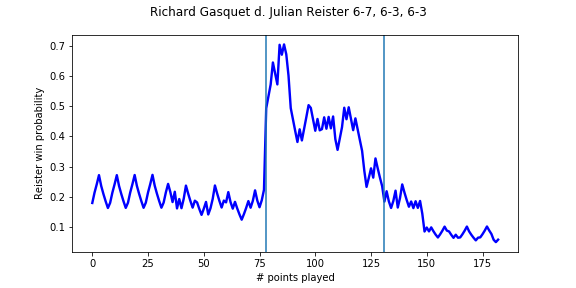
\includegraphics[scale=.7]{gasquet_reister_9_6_all_features}

One drawback of logistic regression is that it cannot distinguish between situations whose score differentials are equivalent. A player serving at (1,1),(5,4),(3,0) will have approximately the same win probability as one serving at (1,1),(1,0),(3,0). However, in the first situation, the player serving wins the match if he wins any of the next three points. From the second scenario, the player serving only holds a break advantage early in the set, from which the returner has many more chances to come back. Assuming each player serves at $f_i=f_j=.64$, our win-probability equation suggests a substantial difference between these two scenarios:

\begin{center}
$P_m(1,1,5,4,3,0) = .994$

$P_m(1,1,1,0,3,0) = .800$
\end{center}

Although the first situation is clearly favorable, logistic regression will compute approximately the same probability in both scenarios $\footnote{\text{after fitting coefficients for the equation P(win) = logit($s_i,s_j,g_i,g_j,{x}_i,{x}_j)= \frac{e^{(c_1s_i+c_2s_j+c_3g_i+c_4g_j+c_5x_i+c_6x_j}}{1+e^{(c_1s_i+c_2s_j+c_3g_i+c_4g_j+c_5x_i+c_6x_j}}$}, coefficients $ c_1 \approx c_2, c_3 \approx c_4,c_5 \approx c_6$ by symmetry and therefore $logit(1,0,5,4,3,0) \approx logit(1,0,1,0dddd,3,0) $}$

%$\footnote{after fitting coefficients for the equation $P(win) = logit(s_i,s_j,g_i,g_j,{x}_i,{x}_j) = \frac{e^{(c_1s_i+c_2s_j+c_3g_i+c_4g_j+c_5x_i+c_6x_j}}{55}$, coefficients $ c_1 \approx c_2, c_3 \approx c_4,c_5 \approx c_6$ by symmetry and therefore}$

Another issue is that logistic regression can fail to detect when a higher-ranked player is about to lose in a close match. Below,

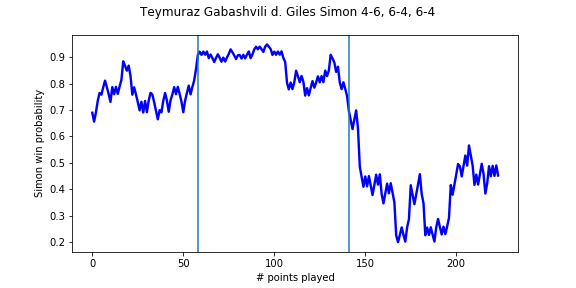
\includegraphics[scale=.7]{simon_gabashvili_9_6_all_features}


\section{Random Forests}
Brian Burke's win-probability models are among the most well-known in sports. They calculate a team's win probability at any point in the match based on historical data through a combination of binning similar scenarios and smoothing probabilities. Nettleton and Lock built on this method by using a random forest approach.

A random forest consists of an ensemble of randomly generated classification trees. Each tree forms decision functions for a subset of features with splits that generate maximum discriminatory ability. Nettleton and Lock also deviate from the traditional random forest classification problem in using regression trees and averaging their estimates to produce a probability estimate, rather than a majority vote.

Then, training on our validation set, we test two random forest models on our point-by-point dataset, one with classification trees and one with regression trees.

\begin{table}[H]
\centering
\caption{Random Forest features}
\label{my-label}
\begin{tabular}{ll}
 \hline
 Variable & Description \\
 \hline
 $surface$ & hard, clay, grass \\
 \hline
 $set$ &  first, second, third \\
 \hline
 $eloDiff$ &  Elo($p_0$) - Elo($p_1$) \\
 \hline
 $setDiff$ &  SetsWon($p_0$) - SetsWon($p_1$)\\
 \hline
 $breakAdv$ &  ServeGamesWon($p_0$) - ServeGamesWon($p_1$) + I(currently serving)\\
 \hline
 $pointDiff$ &  inGamePointsWon($p_0$) - inGamePointsWon($p_1$)\\
 \hline
 $brkPointAdv$ & I(holding break point) - I(facing break point)\\
 \hline
\end{tabular}
\end{table}

\section{Hierarchical Markov Model}
With serving percentages already calculated from historical data, our hierarchical Markov model is well-equipped to produce in-match win probability estimates. Using the analytical equation with players' serving abilities $f_{ij},f_{ji}$, we compute $P_m(s_i,s_j,g_i,g_j,x_i,x_j)$ from every scoreline $(s_i,s_j,g_i,g_j,x_i,x_j)$ in a match. To assess this model's performance, we repeat this on every match in our dataset, testing all estimates of $f_{ij},f_{ji}$ (James-Stein normalized, player-adjusted, elo-induced, surface-specific)

\subsection{Beta Experiments}
The above approaches only take into account the current score and pre-calculated serve percentages when computing win probability. However, in many cases, relevant information may be collected from $P_k$. Consider the following in-match substring, 

$P=``SSSS;RSSSRRSS;SSSS;SRRSRSRSSS;SSSS;RRRSSSRSRSSS;"$

The above sequence demonstrates a current scoreline of three games all. However, $p_i$ has won 12/12 service points, while $p_j$ has won 18/30 service points. If both players continue serving at similar rates, $p_i$ is much more likely to break serve and win the match. Since original forecasts are $f_{ij},f_{ji}$ are based on historical serving percentages, it makes sense that in-match serving percentages may help us better determine each player's serving ability on a given day. To do this, we can update $f_{ij},f_{ji}$ at time $t$ of the match to factor in each player's serving performance thus far in the match.

Bevc explored this method by treating a player's serving percentage $f_{ij}$ as a beta prior which could be updated mid-match to form a posterior serving percentage. The beta distribution is a generalization of the uniform distribution. We often use the beta distribution to represent prior and posterior estimates of some unknown probability $p$. (can include stats notation with beta-binomial conjugacy)

To update our matches with in-match serving statistics, we set $f_{ij}$ as a prior and update with the number of points won and played on $p_i's$ serve, $(s_{won},s_{pt})$. Through beta-binomial conjugacy, we then obtain an update of the form 

$b_{posterior} = \frac{\alpha * f_{ij}+ s_{won}}{\alpha * f_{ij} + s_{pt}}$

where $\alpha$ is a hyperparameter that determines the strength of our prior. Regardless of alpha, the match's influence on our posterior serve estimates always grows as more points have been played.

\subsection{Elo-induced Serve Probabilities}
Earlier on, Klaassen and Magnus suggested a method to infer serving probabilities from a pre-match win forecast $\pi_{ij}$. By imposing a constraint $f_{ij}+f_{ji}=t$, we can then create a one-to-one function 
$S: S(\pi_{ij},t) \rightarrow (f_i,f_j)$, which generates serving probabilities $\hat{f_{ij}},\hat{f_{ji}}$ for both players such that $P_{m}(0,0,0,0,0,0)=\pi_{ij}$ \footnote{$f_{ij}$ and $f_{ji}$ are computed as specified in 3.4 with James-Stein normalization, so as to prevent extreme results}. As this paper was published in 2002, Klaassen and Magnus inverted their match probability equations to produce serve probabilities for ATP rank-based forecasts. However, since elo outperforms ATP rank, we apply this method to elo forecasts.

Due to branching complexity (see section 2.5), our hierarchical Markov model's match probability equation has no analytical solution to its inverse, even when we specify $f_{ij}+f_{ji}=t$. Therefore, we turn to the following approximation algorithm to generate serving percentages that correspond to a win probability within $\epsilon$ of our elo forecast's:

\begin{algorithm}
\caption{elo-induced serve probabilities}\label{euclid}
\begin{algorithmic}[1]
\Procedure{EloInducedServe(prob,sum,$\epsilon$)}{}
\State $\text{s0} \gets \text{sum/2}$
\State $\text{currentProb} \gets \text{.5}$
\State $\text{diff} \gets \text{sum/4}$

\While {$|$currentProb - prob$| > \epsilon $}:

\State $\text{currentProb} \gets \text{matchProb(s0,sum-s0)}$
\If {$\text{currentProb \textless$ $ prob}$}
\State s0 += diff 
\Else
\State s0 -= diff
\EndIf
\State diff = diff/2

\EndWhile


\State \Return s0, sum-s0

\EndProcedure
\end{algorithmic}
\end{algorithm}

To generate elo-induced serve probabilities for a given match, we run the above algorithm with PROB=$\pi_{ij}$, SUM=$f_{ij}+f_{ji}$, and $\epsilon$ set to a desired precision level $\footnote{for purposes of this project, setting $epsilon$=.001 is sufficiently accurate}$. At each step, we call matchProb() to compute the win probability from the start of the match if $p_i$ and $p_j$ had serve probabilities $f_{ij}=s0, f_{ji}=\text{sum}-s0$, respectively. Then we compare currentProb to prob and increment by diff, which halves at every iteration. This process continues until the serve probabilities s0, sum-s0 produce a win probability within $\epsilon$ of PROB, taking $O(\log{\frac{1}{\epsilon}})$ calls to matchProb.

This inverse algorithm is useful for several reasons. Given any effective pre-match forecast $\pi_{ij}$, we can produce serve probabilities that are consistent with $\pi_{ij}$ according to our hierarchical Markov model. By setting the constraint $f_{ij}+f_{ji}=t$, we also ensure that the sum of our players' serve probabilities agrees with historical data. While Klaassen and Magnus argue that $t = f_{ij}+f_{ji}$ is largely independent of $\pi_{ij}$, $t$ holds greater importance when predicting specific score lines a match \cite{Barnett2006}. Using the hierarchical Markov Model's equations, Barnette specifically computed the probability of reaching any set score given parameters $f_{ij},f_{ji}$. When comparing probabilities across matches, one can observe that as $t$ increases, closer set scores and tie-break games become more likely \footnote{``closer'' scores meaning 7-6, 6-7, 7-5, 5-7, etc.}. That is, $t$ encodes information regarding likely trajectories of a match scoreline and relative importance of winning each game on serve. For higher $t$, service games are won more often and service breaks hold relatively higher importance, while the opposite holds for lower $t$. Now, given $\pi_{ij}$ and $t$ \footnote{to avoid extreme values of $t$ from limited player data, this paper uses James-Stein normalized estimates to calculate $t$: $t = JS(f_{ij})+JS(f_{ji})$}, we can produce elo-induced serve probabilities for any two players.





\subsection{Significance of $f_{ij}+f_{ji}$}

To illustrate the importance of maintaining $t=f_{ij}+f_{ji}$, consider the two following matches.

Feliciano Lo'pez v. John Isner (ATP Shanghai 2014, hard court) 

\begin{center}
\begin{tabular}{ |c|c|c|c|c|c|c|c| } 
 \hline
 $p_i$ & $p_j$ & tourney name
 & $\pi_{ij}$ & $t$ & $\#$ r\_points & $g_i$ & elo rating \\ 
 \hline
 Daniel Elahi & 51 & 64 & .7969 & 22 & 67 & .3284 & 1516.9178 
 \\
 \hline
 Ivo Karlovic & 3516 & 4654 & .7555 & 1409 & 4903 & .2874 & 1876.9545 \\ 
 \hline
\end{tabular}
\end{center}

Examples: Federer vs Isner at Paris (or Karlovic vs Isner for more even match), then Ferrer vs. Nishikori/Schwartzman or something with really good returners. (can visualize this with new win probabilities, use example when Karlovic and Schwartzman both had the same win probability)

% write about importance on shape of match

$t$'s influence on the trajectory of a match suggests that prediction from any in-match scoreline will be most effective if serve probabilities are consistent with $t$.

Take two matches with $\pi_{1ij} \approx \pi_{2ij}$. Then graph the matches' WP with respect to a made-up scoreline that includes one service break.

Since elo ratings fail to capture this, it is crucial that we find a way to incorporate this into our model.

show a histogram with sums.

\section{Results}

The following results were tested after training matches on 2011-2013 data and testing on 2014 point-by-point matches (2345). From the training set, we determined that setting hyperparameter $\alpha=200$ yielded optimal performance.

\begin{center}
\begin{tabular}{ |c|c|c| } 
 \hline
 method & accuracy & log loss
   \\ 
 \hline
  LR 1) & 71.5 & .539
  \\ 
 \hline
  LR 2) & 75.4 & .503
  \\ 
 \hline
 LR 3) & 76.4 & .486
  \\ 
 \hline
 Random Forest &  & 
  \\ 
 \hline
 KM James-Stein & 74.9 & .502
  \\ 
 \hline
 KM adjusted James-Stein & 75.5 & .501
  \\ 
 \hline
 KM elo-induced James-Stein & 76.1 & .486
  \\ 
 \hline
  KM logit-induced & 76.4 & .482
  \\ 
 \hline
 KM logit-induced (a=300) & 76.4 & .478
  \\ 
 \hline
\end{tabular}
\end{center}






Results: include a breakdown of performance by surface and set (can compare top models in each category as well).

Mention Variable importance in LR model (serve percentages could be analogous to beta experiments)

What if we took the max(1.1,fij + fji)? There are plenty of matches with freakishly low serving sums calculated from the data






\bibliographystyle{plain}
\bibliography{references}

\end{document}